\documentclass[12pt,a4paper,oneside]{memoir}
\pagestyle{plain}
% Set margins
\usepackage[a4paper, margin=1in]{geometry}

% Add packages for your needs
\usepackage{amsmath, amssymb, mathtools, amsthm}
\usepackage{graphicx, microtype}
\usepackage{natbib}

\usepackage{comment}
\usepackage[utf8]{inputenc}
\usepackage[english]{babel}
\usepackage{float}
\usepackage{lipsum}
\usepackage{csquotes}
\usepackage{subcaption}



\usepackage{algorithm}
\usepackage{algpseudocode}
\usepackage{todonotes}
\usepackage{booktabs}
\usepackage{titlesec}
\usepackage{hyperref}
\usepackage{cleveref}


% Modify appendix
\renewcommand{\appendixname}{Appendix}
\renewcommand*\cftappendixname{\appendixname}

\DeclareMathOperator{\EX}{\mathbb{E}}% expected value
\DeclareMathOperator{\Var}{\mathbb{V}}% Variance

% Define theorem-like environments
\theoremstyle{definition}
\newtheorem{theorem}{Theorem}[chapter]
\newtheorem{lemma}[theorem]{Lemma}
\newtheorem{definition}[theorem]{Definition}	
\newtheorem{example}[theorem]{Example}


% Cleeref setup
\crefname{equation}{Equation}{Equations}
\crefname{theorem}{Theorem}{Theorems}
\crefname{example}{Example}{Examples}


% Define Algorithm as a theorem-like environment
\makeatletter
\let\c@algorithm\c@theorem
\makeatother
\renewcommand{\thealgorithm}{\thetheorem}


% Acronyms
\usepackage{glossaries}
%\makeglossaries

\newacronym{SSM}{SSM}{state-space model}
\newacronym{PMCMC}{PMCMC}{Particle Markov chain Monte Carlo}
\newacronym{IS}{IS}{importance sampling}
\newacronym{SIS}{SIS}{sequential importance sampling}
\newacronym{SISR}{SISR}{sequential importance sampling with resampling}
\newacronym{SMC}{SMC}{sequential Monte Carlo}
\newacronym{SISAR}{SISAR}{sequential Monte Carlo with adaptive resampling}
\newacronym{ESS}{ESS}{Effective Sample Size}
\newacronym{PMMH}{PMMH}{Particle Marginal Metropolis-Hastings}
\newacronym{MCMC}{MCMC}{Markov chain Monte Carlo}
\newacronym{MH}{MH}{Metropolis–Hastings}
\newacronym{LLN}{LLN}{law of large numbers}
\newacronym{MMH}{MMH}{Marginal Metropolis–Hastings}
\newacronym{DGP}{DGP}{data generating process}
\newacronym{FFBSm}{FFBSm}{Forward-Filtering Backward-Sampling}

% Modify chapter title format
\titleformat{\chapter}[hang] 
{\normalfont\huge\bfseries}{\thechapter}{1em}{}

\renewcommand{\appendixname}{Appendix}
\renewcommand*\cftappendixname{\appendixname~}

% Begin the document
\begin{document}
	
	% Custom title page
	\begin{center}
		\vspace*{1cm}
		
		\Huge 
		\textbf{Particle Markov Chain Monte Carlo  Methods}
		
		\vspace{1.5cm}
		
		\textbf{Bjarke Hautop}\\[0.5cm]
		\Large
		Student ID: 202005674
		
		\vspace{1.6cm}
		
\includegraphics[width=0.5\textwidth]{segl.png}
		\vfill
		\Huge
		Master's Thesis in Statistics
		
		\vspace{0.8cm}
		
		
\includegraphics[width=0.4\textwidth]{logo.png}
		
		\Large
		Aarhus University\\
		Supervisor: Jan Pedersen\\
		\today
		
	\end{center}
	\newpage
	
	% Abstract
	%\begin{abstract}
	%	\lipsum[1]
	%\end{abstract}
	\newpage
	
	% Glossary
	%\printglossary[type=main,style=long,nonumberlist]
	%\newpage
	
	% Table of contents
	\tableofcontents*
	
	% Chapter 1: Introduction
	\chapter{Introduction}
	\input{chapters/introduction.tex}
	
	% Chapter 2: Monte Carlo Methods
	\chapter{Monte Carlo Methods}
	\label{chap:MCM}
	In this chapter, we provide the theoretical foundation for \gls*{PMCMC}. We follow the work of \cite{Andrieu}, \cite{Doucet}, and \cite{kroese2013handbook}.

Let $\mu$ be a $\sigma$-finite reference measure on the space $\mathcal{X}$ where each $x_i$ takes values, and denote by $\mu^{\otimes n}$ the corresponding product measure on $\mathcal{X}^n$. Let $x_{1:n} = (x_1, x_2, \dots, x_n)$ and suppose we have a density $\pi_n(x_{1:n})$ (with respect to $\mu^{\otimes n}$) given by
\begin{equation}
	\pi_n(x_{1:n}) = \frac{\gamma_n(x_{1:n})}{Z_n}, \label{eq:density}
\end{equation}
where $\gamma_n(x_{1:n})$ is the unnormalized density and the normalizing constant is defined as
\[
Z_n = \int_{\mathcal{X}^n} \gamma_n(x_{1:n})\, d\mu^{\otimes n}(x_{1:n}).
\]
In many applications and for notational simplicity, we for the rest of this chapter let $\mathcal{X} \subseteq \mathbb{R}^d$ and $\mu$ be the Lebesgue measure, in which case  $Z_n$ is given by
\begin{equation}
	Z_n = \int \gamma_n(x_{1:n})\, dx_{1:n}.
	\label{eq:normalizing_constant}
\end{equation}

Let $X_{1:n}\sim \pi_n(x_{1:n})$ and suppose we generate $N$ i.i.d. samples $x_{1:n}^{(1)},x_{1:n}^{(2)},\dots,x_{1:n}^{(N)}$. We can then approximate $\pi_n(x_{1:n})$ by the empirical measure
\[
{\pi}_n^{\text{MC}}(x_{1:n})=\frac{1}{N} \sum_{i=1}^N \delta_{X_{1:n}^{(i)}}(x_{1:n}),
\]
where $\delta_{X_{1:n}^{(i)}}(x_{1:n})$ denotes the Dirac measure centered at $X_{1:n}^{(i)}$. We can also approximate any marginal $\pi_n(x_k)$ as
\[
{\pi}_n^{\text{MC}}(x_k)=\frac{1}{N} \sum_{i=1}^N \delta_{X_{k}^{(i)}}(x_{k}).
\]
The expectation of any function $H_n: \mathcal{X}^n \to \mathbb{R}$ is given by
\[
I_n(H_n)\coloneq \mathbb{E}_{X_{1:n} \sim \pi_n}[H_n(X_{1:n})]=\int H_n(x_{1:n})\pi_n(x_{1:n})\, dx_{1:n},
\]
and by the \gls*{LLN} we can estimate it by
\[
I_n^{\text{MC}}(H_n) \coloneq \int H_n(x_{1:n})\pi_n^{\text{MC}}(x_{1:n})dx_{1:n}=\frac{1}{N}\sum_{i=1}^NH_n(x_{1:n}^{(i)}).
\]
However, this requires that we can sample from $\pi_n(x_{1:n})$, which often is not the case when it is a complex high-dimensional distribution. 
\section{Importance Sampling}
A way to solve this issue is to use \gls*{IS}. Here we introduce an importance density $q_n(x_{1:n})$ which we can sample from and such that 
\[
\pi_n(x_{1:n})>0 \implies q_n(x_{1:n})>0.
\]
For the remainder of this chapter, we let 
\[
	X_{1:n} \sim q_n(x_{1:n}).
\]
Suppose we generate $N$ i.i.d. samples $x_{1:n}^{(1)},x_{1:n}^{(2)},\dots,x_{1:n}^{(N)}$. 
To correct for the fact that we sample from $q_n$ we define the \emph{unnormalized weight} function
\[
w_n(x_{1:n}) \coloneq \frac{\gamma_n(x_{1:n})}{q_n(x_{1:n})}
\]
and define the \emph{normalized weight} function
\[
W_n^{(i)} \coloneq \frac{w_n(X_{1:n}^{(i)})}{\sum_{j=1}^N w_n(X_{i:n}^{(j)})}.
\]
From \cref{eq:density} and \cref{eq:normalizing_constant} we get
\begin{equation}
	\pi_n(x_{1:n})=\frac{w_n(x_{1:n})q_n(x_{1:n})}{Z_n},
\end{equation}
and
\begin{equation}
	Z_n=\int w_n(x_{1:n})q_n(x_{1:n})\, dx_{1:n}.
\end{equation}
We then define the \gls*{IS} estimators of respectively $\pi_n(x_{1:n})$ and $Z_n$ as
\begin{align}
	\widehat{\pi}_n(x_{1:n}) &= \sum_{i=1}^{N}W_n^{(i)} \delta_{X_{1:n}^{(i)}}(x_{1:n}), \label{eq:est_pi} \\
	\widehat{Z}_n &= \frac{1}{N}\sum_{i=1}^{N}w_n(X_{1:n}^{(i)}). \label{eq:est_Z}
\end{align}
Next, we will show what the relative variance of $\widehat{Z}_n$ is.
\begin{theorem}[Relative variance of $\Var(\widehat{Z}_n)$]
	\label{thm:rel_var_Z_IS}
	The relative variance of the \gls*{IS} estimate of the  normalizing constant $Z_n$ is given by
	\[
	\frac{\Var(\widehat{Z}_n)}{Z_n^2}=\frac{1}{N}\Bigl(\int \frac{\pi_n^2(x_{1:n})}{q_n(x_{1:n})}\, dx_{1:n}-1\Bigr).
	\]
\end{theorem}
\begin{proof}
	The variance of $\widehat{Z}_n$ is 
	\begin{align*}
		\Var(\widehat{Z}_n)&=\frac{1}{N}\Var\bigl(w_n(X_{1:n})\bigr) \\
		&=\frac{1}{N}\Bigl(\EX[w_n^2(X_{1:n})]-\EX[w_n(X_{1:n})]^2\Bigr) \\
		&=\frac{1}{N}\Bigl(\int \frac{\gamma_n^2(x_{1:n})}{q_n^2(x_{1:n})} q_n(x_{1:n})\, dx_{1:n}-Z_n^2\Bigr) \\
		&=\frac{1}{N}\Bigl(\int \frac{\gamma_n^2(x_{1:n})}{q_n(x_{1:n})}\, dx_{1:n}-Z_n^2\Bigr) \\
		&=\frac{1}{N}\Bigl(\int \frac{Z_n^2\pi_n^2(x_{1:n})}{q_n(x_{1:n})}\, dx_{1:n}-Z_n^2\Bigr) \\
		&=\frac{Z_n^2}{N}\Bigl(\int \frac{\pi_n^2(x_{1:n})}{q_n(x_{1:n})}\, dx_{1:n}-1\Bigr).
	\end{align*}
	Dividing by $Z_n^2$ gives the result.
\end{proof}
\noindent Furthermore, we can also estimate $I_n(H_n)$ by
\[
I_n^{\text{IS}}(H_n) \coloneq \int H_n(x_{1:n})\widehat{\pi}(x_{1:n})\, dx_{1:n}=\sum_{i=1}^N W_n^{(i)}H_n(X_{1:n}^{(i)})=\frac{\frac{1}{N}\sum_{i=1}^{N}w_n(X_{1:n}^{(i)})H_n(X_{1:n}^{(i)})}{\frac{1}{N}\sum_{i=1}^{N}w_n(X_{1:n}^{(i)})}.
\]
Note, that the numerator is an unbiased estimate of $Z_nI_n(H_n)$, since
\begin{align*}
	\EX\left[\frac{1}{N}\sum_{i=1}^{N} w_n(X_{1:n}^{(i)})H_n(X_{1:n}^{(i)})\right] &= \EX\Big[w_n(X_{1:n})H_n(X_{1:n})\Big] \\
	&=\int w_n(x_{1:n})H_n(x_{1:n})q(x_{1:n})\, dx_{1:n} \\
	&=\int H_n(x_{1:n})\gamma_n(x_{1:n})\, dx_{1:n} \\
	&=Z_n I_n(H_n).
\end{align*}
Similar calculations gives that the denominator is an unbiased estimate of $Z_n$. Thus, we have a ratio of unbiased estimates, which is not unbiased. However, it is still consistent, which follows by using the \gls*{LLN} and properties of a.s. convergence. 


A natural choice for an importance density $q_n(x_{1:n})$ is one that minimizes the variance of $\widehat{Z}_n$. As shown in \cref{thm:min_var_IS}, this minimum variance is achieved when
\[
q_n(x_{1:n})=\pi_n(x_{1:n}).
\]
However, we cannot select this, as this was the reason we used \gls*{IS} in the first place. Nonetheless, this result indicates that the importance density should closely resemble the target density.

We could now sample from $\pi_n(x_{1:n})$ using the above method. However, to generate a sequence of samples for each $n$, we would have that each step would grow linearly in $n$, as generating samples from $\pi_{n+1}(x_{1:n+1})$ depends on the previous samples up to time $n$. This makes such an algorithm unfeasible in practice. 

\begin{theorem}[Minimum Variance of IS]
	\label{thm:min_var_IS}
	The variance \(\Var[\widehat{Z}_n]\) is minimized if
	\[
	q_n(x_{1:n}) = \pi_n(x_{1:n}) = \frac{\gamma_n(x_{1:n})}{Z_n}.
	\]
\end{theorem}
The proof is done by using Lagrange multiplier, and is inspired by \cite{min_var_IS}.
\begin{proof}
	By independence we have, 
	\[
	\Var[\widehat{Z}_n] = \frac{1}{N}\Var\left[w_n(X_{1:n})\right].
	\]
	We then have   
	\[
	\Var[w_n(X_{1:n})] = \mathbb{E}\left[\frac{\gamma_n(X_{1:n})^2}{q_n(X_{1:n})^2}\right] - Z_n^2
	= \int \frac{\gamma_n(x_{1:n})^2}{q_n(x_{1:n})}\, dx_{1:n} - Z_n^2.
	\]
	Minimizing \(\Var[\widehat{Z}_n]\) is thus equivalent to minimizing
	\[
	J(q_n) = \int \frac{\gamma_n(x_{1:n})^2}{q_n(x_{1:n})}\, dx_{1:n},
	\]
	subject to the constraint
	\[
	\int q_n(x_{1:n})\, dx_{1:n} = 1.
	\]
	We now introduce a Lagrange multiplier \(\lambda\) and form the Lagrangian
	\[
	L(q_n, \lambda) = \int \frac{\gamma_n(x_{1:n})^2}{q_n(x_{1:n})}\, dx_{1:n} 
	+ \lambda \left(\int q_n(x_{1:n})\, dx_{1:n} - 1\right).
	\]
	Taking the functional derivative with respect to \(q_n(x_{1:n})\) and using chain rule we have
	\[
	\frac{\delta L}{\delta q_n(x_{1:n})} = -\frac{\gamma_n(x_{1:n})^2}{q_n(x_{1:n})^2} + \lambda = 0.
	\]
	Solving for \(q_n(x_{1:n})\) yields
	\[
	q_n(x_{1:n}) = \frac{\gamma_n(x_{1:n})}{\sqrt{\lambda}}.
	\]
	Enforcing the normalization condition we get
	\[
	\int \frac{\gamma_n(x_{1:n})}{\sqrt{\lambda}}\, dx_{1:n} = 1 \quad\Longrightarrow\quad \frac{Z_n}{\sqrt{\lambda}} = 1,
	\]
	so that \(\sqrt{\lambda} = Z_n\). Therefore,
	\[
	q_n(x_{1:n}) = \frac{\gamma_n(x_{1:n})}{Z_n} = \pi_n(x_{1:n}).
	\]
	This completes the proof.
\end{proof}
\section{Sequential Importance Sampling}
\Gls*{SIS} builds upon the basic idea of \gls*{IS} by exploiting a Markov structure of the importance distribution. Instead of sampling the full trajectory at once, \gls*{SIS} extends the particle trajectories sequentially, updating the importance weights recursively. This leads to significant computational savings.

We let our importance distribution have a Markov structure, that is
\[
q_n(x_{1:n})=q_1(x_1)q_2(x_2\vert x_1)\dots q_n(x_k\vert x_{1:k-1}),
\]
and each element in the set $\{x_{1:t}\}$ we will refer to as a particle. For $n\geq 2$ define the \emph{incremental importance weight} as
\[
\alpha_n(x_{1:n}) \coloneq \frac{\gamma_n(x_{1:n})}{\gamma_{n-1}(x_{1:n-1})q_n(x_n \vert x_{1:n-1})}.
\]
The unnormalized weights can then be written recursively as 
\begin{align}
	\begin{split}
		\label{eq:unnormalized_weights_recursive}
		w_n(x_{1:n})&=\frac{\gamma_n(x_{1:n})}{q_n(x_{1:n})} \\
		&=\frac{\gamma_{n-1}(x_{1:n-1})}{q_{n-1}(x_{1:n-1})}\frac{\gamma_n(x_{1:n})}{\gamma_{n-1}(x_{1:n-1})q_n(x_n\vert x_{1:n-1})} \\
		&=w_{n-1}(x_{1:n-1})\cdot \alpha_n(x_{1:n})  \\
		&=w_1(x_1) \prod_{k=2}^n \alpha_k(x_{1:k}).
	\end{split}
\end{align}
Summarizing, the \gls*{SIS} method is described in \hyperref[algo:SIS]{Algorithm \ref*{algo:SIS}}, which has a time complexity of $O(NT)$, since the algorithm consists of two nested loops, one over the number of particles $N$, and one over the number of time steps $T$. Within the two nested loops, each operation is $O(1)$.

\begin{algorithm}[H]
	\caption{Sequential Importance Sampling (SIS)}
	\label{algo:SIS}
	\begin{algorithmic}[1]
		\State Generate particles \(x_1^{(i)}\) from  \(q_1(x_1)\) for \( i = 1, \dots, N \)
		\For{each time step \(n = 2, \dots, T\)}
		\For{each particle \( i = 1, \dots, N \)}
		\State Generate particles \(x_n^{(i)}\) from \(q_n(x_n\vert x_{1:n-1}^{(i)})\) 
		\State Compute the incremental importance weight: 
		\[
		\alpha_n^{(i)} = \frac{\gamma_n(x_{1:n}^{(i)})}{\gamma_{n-1}(x_{1:n-1}^{(i)}) q_n(x_n^{(i)} \vert x_{1:n-1}^{(i)})} 
		\] 
		\State Update the particle weight: \( w_n^{(i)} = w_{n-1}^{(i)} \cdot \alpha_n^{(i)} \)
		\EndFor
		\State Normalize the weights: \(W_n^{(i)} \leftarrow \frac{w_n^{(i)}}{\sum_{i=1}^N w_n^{(i)}} \)
		\EndFor
	\end{algorithmic}\\
	% MAKE ALGORITHM MORE LIKE PMMH? I.E. EXPLICIT INPUT OUTPUT
\end{algorithm}
We note, that this algorithm has time complexity $O(NT)$.

However, this method has a severe drawback, that the relative estimated variance $\Var(\widehat{Z}_n)/Z_n^2$ increases exponentially in $n$ even in simple examples. Example \ref{exa:rel_var_IS_explodes} illustrates this issue.
\begin{example}\label{exa:rel_var_IS_explodes}
	Consider the case where $\mathcal{X}=\mathbb{R}$ and let the density $\pi_n(x_{1:n})$ be given by
	\[
	\pi_n(x_{1:n})=\prod_{k=1}^n \pi_n(x_k)=\prod_{k=1}^n \frac{1}{\sqrt{2\pi}}\exp\Bigl(-\frac{x_k^2}{2}\Bigr).
	\]
	Thus, the unnormalized density $\gamma_n(x_{1:n})$ is given by
	\[
	\gamma_n=\prod_{k=1}^n \exp\Bigl(-\frac{x_k^2}{2}\Bigr),
	\]
	and the normalizing constant $Z_n$ is
	\[
	Z_n=(2\pi)^{n/2}.
	\]
	Ignoring that we could easily sample from $\pi_n$, we select the importance distribution $q_n$ to sample from as
	\[q_n(x_{1:n})=\prod_{k=1}^n \pi_n(x_k)=\prod_{k=1}^n \frac{1}{\sqrt{2\pi\sigma^2}}\exp\Bigl(-\frac{x_k^2}{2\sigma^2}\Bigr)\]
	and we are interested in estimating $Z_n$. Recall from \cref{thm:rel_var_Z_IS} that the relative variance of $\widehat{Z}_n$ is given by
	\[
	\frac{\Var(\widehat{Z}_n)}{Z_n^2}=\frac{1}{N}\Bigl(\int \frac{\pi_n^2(x_{1:n})}{q_n(x_{1:n})}\, dx_{1:n}-1\Bigr).
	\]
	In our case this factors over the coordinates and we have
	\begin{align*}
		\int \frac{\pi_n(x_{1:n})^2}{q_n(x_{1:n})}\, dx_{1:n}&=\prod_{k=1}^{n}\int \frac{1/(2\pi)\exp(-x^2)}{1/\sqrt{2\pi\sigma^2}\exp(-x^2/(2\sigma^2))}\, dx_{1:k} \\
		&=\biggl[\frac{\sqrt{2\pi\sigma^2}}{2\pi}\int \exp\Bigl(-x^2+\frac{x^2}{2\sigma^2}\Bigr)\, dx \biggr]^n \\
		&=\biggl[\frac{\sqrt{2\pi\sigma^2}}{2\pi}\int \exp\Bigl(-\Bigl(1-\frac{1}{\sigma^2}\Bigr)x^2\Bigr)\, dx \biggr]^n.
	\end{align*}
	The integral is finite if and only if $1-1/(2\sigma^2)>0$, that is $\sigma^2>1/2$. In this case, it is equal to 
	\[
	\int_{-\infty}^{\infty} \exp\Bigl(-\Bigl(1-\frac{1}{\sigma^2}\Bigr)x^2\Bigr)\, dx=\sqrt{\frac{\pi}{1-1/(2\sigma^2)}}.
	\]
	Thus, for $\sigma^2>1/2$ we have
	\begin{align*}
		\int \frac{\pi_n(x_{1:n})^2}{q_n(x_{1:n})}\, dx_{1:n} &=\biggl(\frac{\sqrt{2\pi\sigma^2}}{2\pi} \sqrt{\frac{\pi}{1-1/(2\sigma^2)}}\biggr)^n \\
		&=\biggl(\sqrt{\frac{\sigma^4}{2\sigma^2-1}}\biggr)^n \\
		&=\Bigl(\frac{\sigma^4}{2\sigma^2-1}\Bigr)^{n/2}.
	\end{align*}
	Finally, we can conclude that for $\sigma^2>1/2$ the relative variance becomes $\Var[\widehat{Z}_n]<\infty$ and 
	\[
	\frac{\Var[\widehat{Z}_n]}{Z_n^2}=\frac{1}{N}\biggl[\Bigl(\frac{\sigma^4}{2\sigma^2-1}\Bigr)^{n/2}-1\biggr].
	\]
	Note that for any $1/2<\sigma^2\neq 1$ we have that $\sigma^4/(2\sigma^2-1)>1$, and thus the variance increases exponentially with $n$. 
	
	For example, choosing $\sigma^2=1.2$ then we have a reasonably good importance distribution as $q_k(x_k) \approx \pi_n(x_k)$. However,  
	\[
	N\Var[\widehat{Z}_n]/Z_n^2\approx (1.103)^{n/2},
	\]
	which for $n=1000$ is roughly equal to $1.9\cdot 10^{21}$. So we would need to use $N\approx 2\cdot 10^{23}$ particles to obtain a relative variance of $0.01$.
\end{example}

\section{Resampling}
Over time, many particles receive negligible weight, leading to a situation where only a few particles dominate the estimate. This phenomenon, known as weight degeneracy, can degrade the performance of the estimator (\cite{Doucet2000}).
The idea for resampling is to get rid of particles with low weights with a high probability, so the focus is spent on high-probability regions instead of carrying forward particles with very low weights. This typically reduces the variance, see for instance Example \ref{exa:rel_var_IS_explodes_cont}. 
% Also referred to as Bootstrap filter.

The \gls*{IS} approximation \( \widehat{\pi}_n(x_{1:n}) \) of the target distribution \( \pi_n(x_{1:n}) \) is constructed using weighted samples drawn from \( q_n(x_{1:n}) \), meaning that these samples are not distributed according to \( \pi_n(x_{1:n}) \). To obtain a new set of samples that better approximates \( \pi_n(x_{1:n}) \), we employ resampling, where each particle \( X_{1:n}^{(i)} \) is selected with probability proportional to its normalized weight \( W_n^{(i)} \). 

A simple resampling strategy is multinomial resampling, where the number of offspring \( N_n^{(i)} \) assigned to each particle \( X_{1:n}^{(i)} \) follows a multinomial distribution:
\[
N_n^{(1:N)} = (N_n^{(1)},\dots, N_n^{(N)}) \sim \text{Multinomial}(N, W_n^{(1:N)}).
\]
That is, each particle is independently resampled \( N \) times, with probabilities given by the normalized weights \( W_n^{(i)} \).

After resampling, all particles are assigned equal weight, since the resampled particles are now an unweighted representation of the target distribution. Each selected particle appears with frequency \( N_n^{(i)} \), and thus the empirical distribution assigns equal mass to all \( N \) retained particles. That is, the original weighted particle approximation of the target distribution is  
\[
\hat{p}(x) = \sum_{i=1}^{N} W_n^{(i)} \delta_{X_{1:n}^{(i)}}(x),
\]  
and after resampling, the new approximation is  
\[
\hat{p}^*(x) = \sum_{i=1}^{N} \frac{N_n^{(i)}}{N} \delta_{X_{1:n}^{(i)}}(x).
\]  
Taking expectations we obtain
\[
\mathbb{E} \left[ \hat{p}^*(x) \right] = \sum_{i=1}^{N} \mathbb{E} \left[ \frac{N_n^{(i)}}{N} \right] \delta_{X_{1:n}^{(i)}}(x) = \sum_{i=1}^{N} W_n^{(i)} \delta_{X_{1:n}^{(i)}}(x) = \hat{p}(x),
\]  
showing that the resampled particle system should have equal weights to be unbiased. 

Using the recursive structure of the unnormalized weights from \cref{eq:unnormalized_weights_recursive} a natural way to estimate 
$Z_n$ is to define 
\[
\widetilde{Z}_1\coloneq \frac{1}{N}\sum_{i=1}^N w_1(x_1^{i}),
\]
and for $n\geq 2$ estimate $Z_n$ recursively by 
\begin{equation}
	\widetilde{Z}_n \coloneq\widetilde{Z}_{n-1}{\alpha}_n^{\text{MC}}, \label{eq:est_Z_SIS}
\end{equation}
where ${\alpha}_n^{\text{MC}}$ is the standard MC estimate of $\alpha_n$. 

A generic \gls*{SISR} algorithm is given in \hyperref[algo:SISR]{Algorithm \ref*{algo:SISR}}. The time complexity of this algorithm is \(O(NT)\), since it consists of two nested loops, one over the number of particles \(N\), and one over the number of time steps \(T\). Within the nested loops, each operation is \(O(1)\). The resampling step, which involves drawing \(N\) indices according to the particle weights, is done within the \(T\)-loop and has a time complexity of \(O(N)\). Therefore, the overall time complexity is \(O(NT + NT) = O(NT)\).

\begin{algorithm}[H]
	\caption{Sequential Importance Sampling with Resampling (SISR)}
	\label{algo:SISR}
	\begin{algorithmic}[1]
		\State Generate particles \(x_1^{(i)}\) from \( q_1(x_1)\) for \( i = 1, \dots, N \)
		\For{each time step \(n = 2, \dots, T\)}
		\For{each particle \( i = 1, \dots, N \)}
		\State Generate particles \(x_n^{(i)}\) from \(q_n(x_n\vert x_{1:n-1}^{(i)})\) 
		\State Compute the incremental importance weight: 
		\[
		\alpha_n^{(i)} = \frac{\gamma_n(x_{1:n}^{(i)})}{\gamma_{n-1}(x_{1:n-1}^{(i)}) q_n(x_n^{(i)} \vert x_{1:n-1}^{(i)})} 
		\] 
		\State Update the particle weight: \( w_n^{(i)} = w_{n-1}^{(i)} \cdot \alpha_n^{(i)} \)
		\EndFor
		\State Normalize the weights: \(W_n^{(i)} \leftarrow \frac{w_n^{(i)}}{\sum_{i=1}^N w_n^{(i)}} \)
		\State Draw \(N\) indices \(\{a^{(i)}\}_{i=1}^N\) from \(\{1,\dots,N\}\) according to the probabilities \(\{W_n^{(i)}\}\)
		\State Set \( X_{1:n}^{(i)} \leftarrow X_{1:n}^{(a^{(i)})} \) for all \( i \)
		\State Reset weights: $w_n^{(i)}=1$
		\EndFor
	\end{algorithmic}
	% MAKE ALGORITHM MORE LIKE PMMH? I.E. EXPLICIT INPUT OUTPUT
\end{algorithm}
While resampling effectively eliminates low-weight particles, it also causes many distinct trajectories to vanish over successive iterations. In effect, resampling resets the system by providing a reliable approximation of the current state's marginal distribution, albeit at the cost of losing detailed ancestral information. The deeper problem of weight degeneracy is that trying to represent a high-dimensional distribution with a finite number of samples will inevitably fail. 

An alternative would be to increase the number of particles at each iteration; however, this approach quickly becomes infeasible due to the exponential growth in the required number of particles (\cite{Doucet}).

Now we provide a result similar to \cref{thm:rel_var_Z_IS} for the case with resampling. 

\begin{theorem}[Relative Asymptotic Variance with Resampling]
	\label{thm:rel_asym_var_resampling}
	The relative asymptotic variance of the \gls*{IS} estimate of the normalizing constant \(Z_n\) with resampling at every time step is
	\[
	\frac{\Var(\widetilde{Z}_n)}{Z_n^2}=\frac{1}{N}\left[\left(\int 	\frac{\pi_1^2(x_1)}{q_1(x_1)}\,dx_1-1\right)+\sum_{k=2}^n\left(\int \frac{\pi_k^2(x_{1:k})}{\pi_{k-1}(x_{1:k-1})\,q_k(x_k\vert x_{1:k-1})}\,dx_{k-1:k}-1\right)\right].
	\]
\end{theorem}
A proof is omitted but follows from the Feynman–Kac framework; see, e.g., Chapter 9 in \cite{moral2004feynman} for a proof.

Notably, comparing \cref{thm:rel_asym_var_resampling} with \cref{thm:rel_var_Z_IS} reveals that while resampling introduces additional variance, the resampling has a resetting property of the systems. Thus, we get that the associated errors accumulate linearly rather than multiplicatively. This becomes important when the dimension becomes large. We continue Example \ref{exa:rel_var_IS_explodes} using \cref{thm:rel_asym_var_resampling} to highlight this.
\begin{example}[Example \ref{exa:rel_var_IS_explodes} continued]
	\label{exa:rel_var_IS_explodes_cont}
	Using \cref{thm:rel_asym_var_resampling} and using the derivation done in Example \ref{exa:rel_var_IS_explodes} we have that it is finite for $\sigma^2>1/2$ and the relative variance using resampling at every time step is approximately equal to
	\begin{align*}
		\frac{\Var(\widetilde{Z}_n)}{Z_n^2}&\approx\frac{1}{N}\left[\left(\int 	\frac{\pi_1^2(x_1)}{q_1(x_1)}\,dx_1-1\right)+\sum_{k=2}^n\left(\int \frac{\pi_k^2(x_{1:k})}{\pi_{k-1}(x_{1:k-1})\,q_k(x_k\vert x_{1:k-1})}\,dx_{k-1:k}-1\right)\right] \\
		&=\frac{n}{N}\left[\left(\frac{\sigma^4}{2\sigma^2-1}^{1/2}\right)-1\right]
	\end{align*}
	which is linear in $n$ in contrast to the exponential growth of the \gls*{IS} estimate of the relative variance. If we again select $\sigma^2=1.2$ then to obtain a relative variance of $0.01$ we only need $N\approx 10^4$ particles instead of the $N\approx 2\cdot 10^{23}$ particles that were needed for the IS estimate to obtain the same precision. That is, we obtain an improvement by 19 orders of magnitude.
\end{example} 
This setup favors SMC massively since the density $\pi_n(x_{1:n})$) factorizes. A more realistic example is given in Example \ref{exa:SSM_known_theta}.

\subsection{Reducing variance of Resampling}
While resampling helps mitigate weight degeneracy by focusing computational effort on high-probability regions, it introduces additional variance into the algorithm. We describe two distinct techniques that can reduce this extra variance, thereby improving the overall efficiency of the \gls*{SISR} algorithm. Notably, these approaches are complementary and can be applied simultaneously.

We can reduce the variance introduced during resampling by changing the sampling scheme. Several methods exists, but we will focus on stratified resampling, a method often used in survey sampling \cite{kiderlen2022survey}. In stratified resampling, the interval $[0,1]$ is divided into $N$ equal strata, and one uniform random number is drawn from each sub-interval. That is, for $i=1,\dots,N$, we draw 
\[
u_i \sim \text{Uniform}\left(\frac{i-1}{N}, \frac{i}{N}\right).
\]
Each $u_i$ is then used to select a particle based on the cumulative normalized weights. In \cite{douc2005comparisonresamplingschemesparticle} it was shown that stratified resampling always gives lower variance than multinomial resampling. 

% Add systematic resampling?

Another way to reduce the variance of the \gls*{SISR} algorithm is to only do the resampling step when we have many particles with low weights. We will call this \gls*{SISAR}.
A common metric used to decide when to trigger a resampling step is the \emph{effective sample size} (ESS), first introduced by \cite{Liu}. The ESS at time $n$ is defined as
\[
\text{ESS}_n \coloneq \frac{1}{\sum_{i=1}^N \left(W_n^{(i)}\right)^2}\,.
\]
ESS can take a value between $1$ and $N$. When the ESS falls below a predetermined threshold, $N_\tau$, often chosen as $N_\tau=N/2$, it is an indication that most of the weight is carried by only a few particles, and resampling is then warranted.

Thus, the \gls*{SISAR} Algorithm is just the \gls*{SISR} Algorithm described in \cref{algo:SISR} where the resampling is only done when the resampling condition is met. A generic algorithm incorporating adaptive resampling is described in \hyperref[algo:SISAR]{Algorithm \ref*{algo:SISAR}}. The time complexity remains $O(NT)$.
\begin{algorithm}[H]
	\caption{Sequential Importance Sampling with Adaptive Resampling (SISAR)}
	\label{algo:SISAR}
	\begin{algorithmic}[1]
		\State Generate particles \(x_1^{(i)}\) from \( q_1(x_1)\) for \( i = 1, \dots, N \)
		\For{each time step \(n = 2, \dots, T\)}
		\For{each particle \( i = 1, \dots, N \)}
		\State Generate particles \(x_n^{(i)}\) from \(q_n(x_n\vert x_{1:n-1}^{(i)})\) 
		\State Compute the incremental importance weight: 
		\[
		\alpha_n^{(i)} = \frac{\gamma_n(x_{1:n}^{(i)})}{\gamma_{n-1}(x_{1:n-1}^{(i)}) q_n(x_n^{(i)} \vert x_{1:n-1}^{(i)})} 
		\] 
		\State Update the particle weight: \( w_n^{(i)} = w_{n-1}^{(i)} \cdot \alpha_n^{(i)} \)
		\EndFor
		\State Normalize the weights: \(W_n^{(i)} \leftarrow \frac{w_n^{(i)}}{\sum_{i=1}^N w_n^{(i)}} \)
		\If{Resampling condition is met}
		\State Draw \(N\) indices \(\{a^{(i)}\}_{i=1}^N\) from \(\{1,\dots,N\}\) according to the probabilities \(\{W_n^{(i)}\}\)
		\State Set \( x_{1:n}^{(i)} \leftarrow x_{1:n}^{(a^{(i)})} \) for all \( i \)
		\State Reset weights: $w_n^{(i)}=1$
		\EndIf
		\EndFor
	\end{algorithmic}
	% MAKE ALGORITHM MORE LIKE PMMH? I.E. EXPLICIT INPUT OUTPUT
\end{algorithm}
\noindent Again, we can at any step $n$ estimate $Z_n$ by \cref{eq:est_Z_SIS}. 

	% Chapter 3: Review of Particle Markov Chain Monte Carlo Methods
	\chapter{State-Space Models}
	%As a Definition?
\todo{Rewrite}
Suppose we have a hidden Markov model (HMM), also called a state-space model (SSM). Specifically, we consider a discrete-time Markov process $\{X_n; n\geq 1\}$, where  $X_n \subset \mathcal{X}^n$ for each $n$. It is characterized by an initial distribution 
\[
X_1 \sim \mu(x_1)
\] 
and the transition density
\[
X_{n+1} \vert (X_n=x_n) \sim f_\theta(x_{n+1} \vert x_n)
\]
for some parameter $\theta \in \Theta$. Our goal is to infer the latent states $\{X_n\}$, given a sequence of noisy observations $\{Y_n; n\geq 1\}$, where $Y_n \subset \mathcal{Y}^n$ for each $n$. The observation $Y_n$ is assumed to be conditionally independent given $X_n$, meaning that for $1\leq n\leq m$,
\[
Y_n \vert (X_1=x_1,\dots, X_n=x_n,\dots,X_m=x_m) \sim g_\theta(y_n \vert X_n=x_n).
\]
% EXPAND BELOW
Let $y_{1:T}=(y_1,\dots,y_T)$ denote the sequence of observations up to time $T\geq 1$. If $\theta\in \Theta$ is known then Bayesian inference gives us the posterior density as $p_\theta(x_{1:T} \vert y_{1:T}) \propto p_\theta(x_{1:T}, y_{1:T})$ where
\[
p_\theta(x_{1:T}, y_{1:T})=\mu_\theta(x_1)\prod_{n=2}^{T}f_\theta(x_n\vert x_{n-1})\prod_{n=1}^{T}g_\theta(y_n \vert x_n).
\]
When $\theta$ is unknown we give a prior density $p(\theta)$ to $\theta$ and Bayesian inference then relies on the joint posterior density
\[
p(\theta,x_{1:T}\vert y_{1:T}) \propto p_\theta(x_{1:T}, y_{1:T})p(\theta). 
\]
In most cases, neither $p_\theta(x_{1:T}, y_{1:T})$ nor $p(\theta,x_{1:T}\vert y_{1:T})$ admit closed-form solutions, necessitating the use of Monte Carlo methods for inference. In most cases, directly sampling the densities 
is infeasible due to the high-dimensional nature of the state space and the complexity of the model. In the case of a known $\theta \in \Theta$ sequential Monte Carlo (SMC) is a class of algorithms to approximate sequentially the
sequence of posterior densities $\{p_\theta(x_{1:n}\vert y_{1:n}; n\geq 1)\}$ and the sequence of marginal likelihoods $\{p_\theta(y_{1:n}); n\geq 1\}$.

% Apply SMC in this context
SMC methods are a general class of Monte Carlo methods that sample sequentially from a sequence of target
probability densities $\{\pi_n(x_{1:n}); n\geq 1\}$, where $\pi_n(x_{1:n}) \subset \mathcal{X}^n$ for each $n$. 
In many practical applications, the normalizing constant $Z_n$ is unknown, and one of the advantages of SMC is that it also provides an estimate $\widehat{Z}_n$ alongside approximations of the target distribution.
Specifically, at time $n=1$ we get an approximation of $\pi_1(x_1)$ and an estimate of $Z_1$, then at time $n=2$ we get an approximation of $\pi_2(x_{1:2})$ and an estimate of $Z_2$ and so on. Here for instance we could have $\gamma_n(x_{1:n})=p(x_{1:n}, y_{1:n})$ and $Z_n=p(y_{1:n})$, thus $\pi_n(x_{1:n})=p(x_{1:n}\vert y_{1:n})$.

% Filtering+Smoothing? Before or after this?
\section{Filtering}

	
	% Chapter 3: Methodology and Implementation
	%\chapter{Methodology and Implementation}
	%\input{chapters/methodology.tex}
	
	\chapter{Bayesian Inference}
	This chapter builds on the work of \cite{gettingstarted}, \cite{DoucetEstParamSSM} and \dots \todo{cite}. We will purely focus on off-line methods, that is estimating $p(x_{0:T}, \theta \vert y_{0:T})$. 

In many state-space models, both the parameters $\theta$ and the latent states $x_{1:T}$ are unknown and must be inferred simultaneously. In the previous chapter, we used the notation $p_\theta(\cdot)$ to indicate a density dependent on the parameter $\theta$. In this chapter we will use the more explicit notation $p(\cdot\vert \theta)$, as it aligns more naturally with the Bayesian framework.

In a Bayesian framework, a prior distribution $p(\theta)$ is assigned to the parameters, and inference is carried out on the joint posterior distribution given the observations $y_{1:T}$:
\begin{align}
	p(\theta,x_{1:T}\mid y_{1:T}) &= \frac{p(y_{1:T} \vert \theta, x_{1:T})\, p(\theta, x_{1:T})}{p(y_{1:T})} \nonumber \\
	&= \frac{p(y_{1:T} \vert \theta, x_{1:T})\, p(\theta)\, p(x_{1:T}\mid \theta)}{p(y_{1:T})} \nonumber \\
	&= \frac{p(y_{1:T} \vert \theta, x_{1:T})\, p(\theta)\, p(x_{1:T}\mid \theta)}{p(y_{1:T})} \nonumber \\
	&\propto p(y_{1:T} \vert \theta, x_{1:T})\, p(\theta)\, p(x_{1:T}\mid \theta),
	\label{eq:joint-posterior}
\end{align}
where 
\[
	p(y_{1:T})=\int \int p(y_{1:T}\vert \theta, x_{1:T})p(\theta)p(x_{1:T}\vert \theta)\, dx_{1:T}\, d\theta
\] 
is dropped since it is just a normalizing constant. Using the Markov structure of the \gls*{SSM} we can simplify $p(x_{1:T} \vert \theta)$ as
\[
	p(x_{1:T} \vert \theta)=p(x_1 \vert \theta)\prod_{t=2}^{T}p(x_t\vert x_{t-1}\vert \theta).
\]

When the latent states are not of primary interest, they can be integrated out to obtain the marginal posterior for the parameters:
\begin{align}
	p(\theta\mid y_{1:T}) &= \int p(\theta,x_{1:T}\mid y_{1:T})\,dx_{1:T} \nonumber \\
	&\propto p(\theta)\, p(y_{1:T} \vert \theta),
	\label{eq:marginal-posterior}
\end{align}
with the marginal likelihood defined as
\[
p(y_{1:T}\vert \theta) = \int p(x_{1:T}, y_{1:T}\vert \theta)\,dx_{1:T}.
\]

Since neither Equation (\ref{eq:joint-posterior}) or (\ref{eq:marginal-posterior}) is generally tractable, \gls*{MCMC} methods are widely used to approximate the posterior distributions. However, standard techniques such as one-variable-at-a-time Gibbs sampling tend to perform poorly for non-linear, non-Gaussian state-space models \cite{DoucetEstParamSSM}. 

\gls*{PMCMC} algorithms overcome these challenges by leveraging particle methods to construct efficient high-dimensional proposal distributions, thereby enhancing the performance of MCMC in these complex settings.

\subsection{Particle Marginal Metropolis-Hastings (PMMH)}
A \gls*{MMH} sampler would sample from the joint posterior $p(x_{1:T}, \theta \vert y_{1:T})$ by using the proposal density
\begin{equation}
	q\bigl((x_{1:T}', \theta') \vert x_{1:T}, \theta\bigr)=q(\theta'\vert \theta)p_{\theta'}(x_{1:T}' \vert y_{1:T}'),
\end{equation}
where $q(\theta' \vert \theta)$ is a proposal density to obtain a candidate parameter $\theta'$ from $\theta$, a candidate latent trajectory $x_{1:T}'$ from $x_{1:T}$, and an observation trajectory $y_{1:T}'$ from $y_{1:T}$. The acceptance probability is given by
\begin{equation}
	1 \wedge \frac{p_{\theta'}(y_{1:T})p(\theta')q(\theta \vert \theta')}{p_\theta(y_{1:T})p(\theta)q(\theta' \vert \theta)}.
\end{equation}
However, we can neither sample exactly from $p_{\theta'}(x_{1:T}' \vert y_{1:T}')$ nor compute the likelihood terms $p_{\theta'}(y_{1:T})$ and $p_{\theta}(y_{1:T})$ from the acceptance probability an implementation of \gls*{MMH} is impossible. 

A \gls*{PMMH} sampler is an approximation of the \gls*{MMH} sampler where particle methods are used to approximate these intractable terms. The pseudocode for the algorithm is given in Algorithm~\ref{algo:PMMH}. It was shown in \cite{Andrieu} that using an unbiased estimator of $\widehat{p}_\theta(y_{1:T})$ produced by the particle filter is sufficient to guarantee that the Markov chain has the correct stationary distribution for any number of particles $N$. 
% Highlight this? Very important

The proposal density $q(\theta'\vert \theta)$ is often chosen as a random walk, that is $\theta'$ 
\[q(\theta' \vert \theta) \sim N(\theta, \hat{\mathcal{P})},\]
where $\hat{\mathcal{P}}$ is the estimated posterior covariance based on a pilot run (\cite{gettingstarted}).

\begin{algorithm}[H]
	\caption{Particle Marginal Metropolis-Hastings (PMMH)}
	\label{algo:PMMH}
	\begin{algorithmic}[1]
		\State \textbf{Input:} Observation sequence \(y_{1:T}\); number of MCMC iterations \(M\); number of particles \(N\); prior density \(p(\theta)\); proposal density \(q(\theta'\mid\theta)\); and initial parameter value \(\theta^{(0)}\).
		\State \textbf{Initialization:} Set \(m \gets 0\). Run a particle filter (as explained in Chapter~\ref{chap:MCM}) with parameter \(\theta^{(0)}\) to obtain a likelihood estimate \(\widehat{p}_{\theta^{(0)}}(y_{1:T})\) and a latent state sample \(x_{1:T}^{(0)}\).
		\For{\(m=1,\dots,M\)}
		\State Propose a new parameter: \(\theta' \sim q(\theta'\mid\theta^{(m-1)})\).
		\State Run a particle filter with \(\theta'\) to obtain the likelihood estimate \(\widehat{p}_{\theta'}(y_{1:T})\) and a latent state sample \(x_{1:T}'\).
		\State Compute the acceptance probability
		\[
		\alpha = \min\Biggl\{1,\;\frac{p(\theta')\,\widehat{p}_{\theta'}(y_{1:T})\,q(\theta^{(m-1)}\mid\theta')}{p(\theta^{(m-1)})\,\widehat{p}_{\theta^{(m-1)}}(y_{1:T})\,q(\theta'\mid\theta^{(m-1)})}\Biggr\}.
		\]
		\State With probability \(\alpha\), set
		\[
		\theta^{(m)}\gets \theta',\quad x_{1:T}^{(m)}\gets x_{1:T}',\quad \widehat{p}_{\theta^{(m)}}(y_{1:T})\gets \widehat{p}_{\theta'}(y_{1:T}).
		\]
		\State Otherwise, set
		\[
		\theta^{(m)}\gets \theta^{(m-1)},\quad x_{1:T}^{(m)}\gets x_{1:T}^{(m-1)},\quad \widehat{p}_{\theta^{(m)}}(y_{1:T})\gets \widehat{p}_{\theta^{(m-1)}}(y_{1:T}).
		\]
		\EndFor	
		\State \textbf{Return:} The chain \(\{\theta^{(m)},\, x_{1:T}^{(m)}\}_{m=0}^{M}\).
	\end{algorithmic}
\end{algorithm}
Recall, that the particle filter algorithms discussed in Chapter~\ref{chap:MCM} had time complexity $O(NT)$, and thus this algorithm has time complexity $O(MNT)$. Thus, we need to decide on how to allocate computational resources for $N$ and $M$. 

The parameter \(N\) directly impacts the variance of the likelihood estimator \(\widehat{p}_\theta(y_{1:T})\). Increasing \(N\) reduces this variance, leading to a more stable acceptance probability. In practice, $N$ is typically determined via pilot runs that monitor the variance of the log-likelihood estimate, with the common guideline being to choose $N$ so that this variance is approximately around 1-1.7 when evaluated at the posterior mean of $\theta$ (\cite{Pitt} and \cite{gettingstarted}).

The number of MCMC iterations \(M\) determines the overall length of the Markov chain and hence the quality of the posterior approximation. A larger \(M\) facilitates a more thorough exploration of the posterior distribution, allowing for greater precision in the resulting parameter estimates after discarding an appropriate burn-in period. In practice, we often run several independent chains and use convergence diagnostics such as the potential scale reduction statistic, \(\hat{R}\), and the effective sample size of each parameter, see also Appendix~\ref{chp:appendixMCMC}. 


\begin{example}[SSM with unknown $\theta$]
	\label{exa:SSM_unknown_theta}
	We consider the same model from Example~\ref{exa:SSM_known_theta} and Example~\ref{exa:SSM_known_theta_cont}, that is we have $\theta=(\phi, \sigma_x, \sigma_y)$ and we have the following \gls*{SSM}
	\begin{align*}
		X_1 &\sim N(0,\, 1) \\
		X_t&=\phi X_{t-1}+\sin(X_{t-1})+\sigma_x V_t, \quad V_t \sim N(0, \, 1) \\
		Y_t&=X_t+\sigma_y W_t, \quad W_t \sim N(0, \, 1).
	\end{align*}
	We as before, set $\phi=0.7, \sigma_x=1, \sigma_y=1$, with a time horizon of $T=50$, and $N=1000$ particles. We assume $\theta$ is unknown. Thus, we need to specify priors on these three parameters. We choose the following generic weakly informative priors
	\begin{align*}
		\phi &\sim N(0,1), \\
		\sigma_x &\sim \text{half-}N(1), \\
		\sigma_y &\sim \text{half-}N(1).
	\end{align*}
	We do a prior predictive check, where we generate data from the prior and assess whether it aligns with the observed data. Data simulated from the \gls*{DGP} using the true values $\theta=(0.7, 1, 1)$ and four times from the prior is visualized in Figure~\ref{fig:Prior_predictive_check}. We see that the priors are reasonable, but note that if $\lvert \phi \rvert>1$ by the nature of the \gls*{DGP} that the observations can easily explode.  
	
	% Should I define prior predictive check and posterior predictive check?
	\begin{figure}
		\centering
		\textbf{Prior predictive check}
		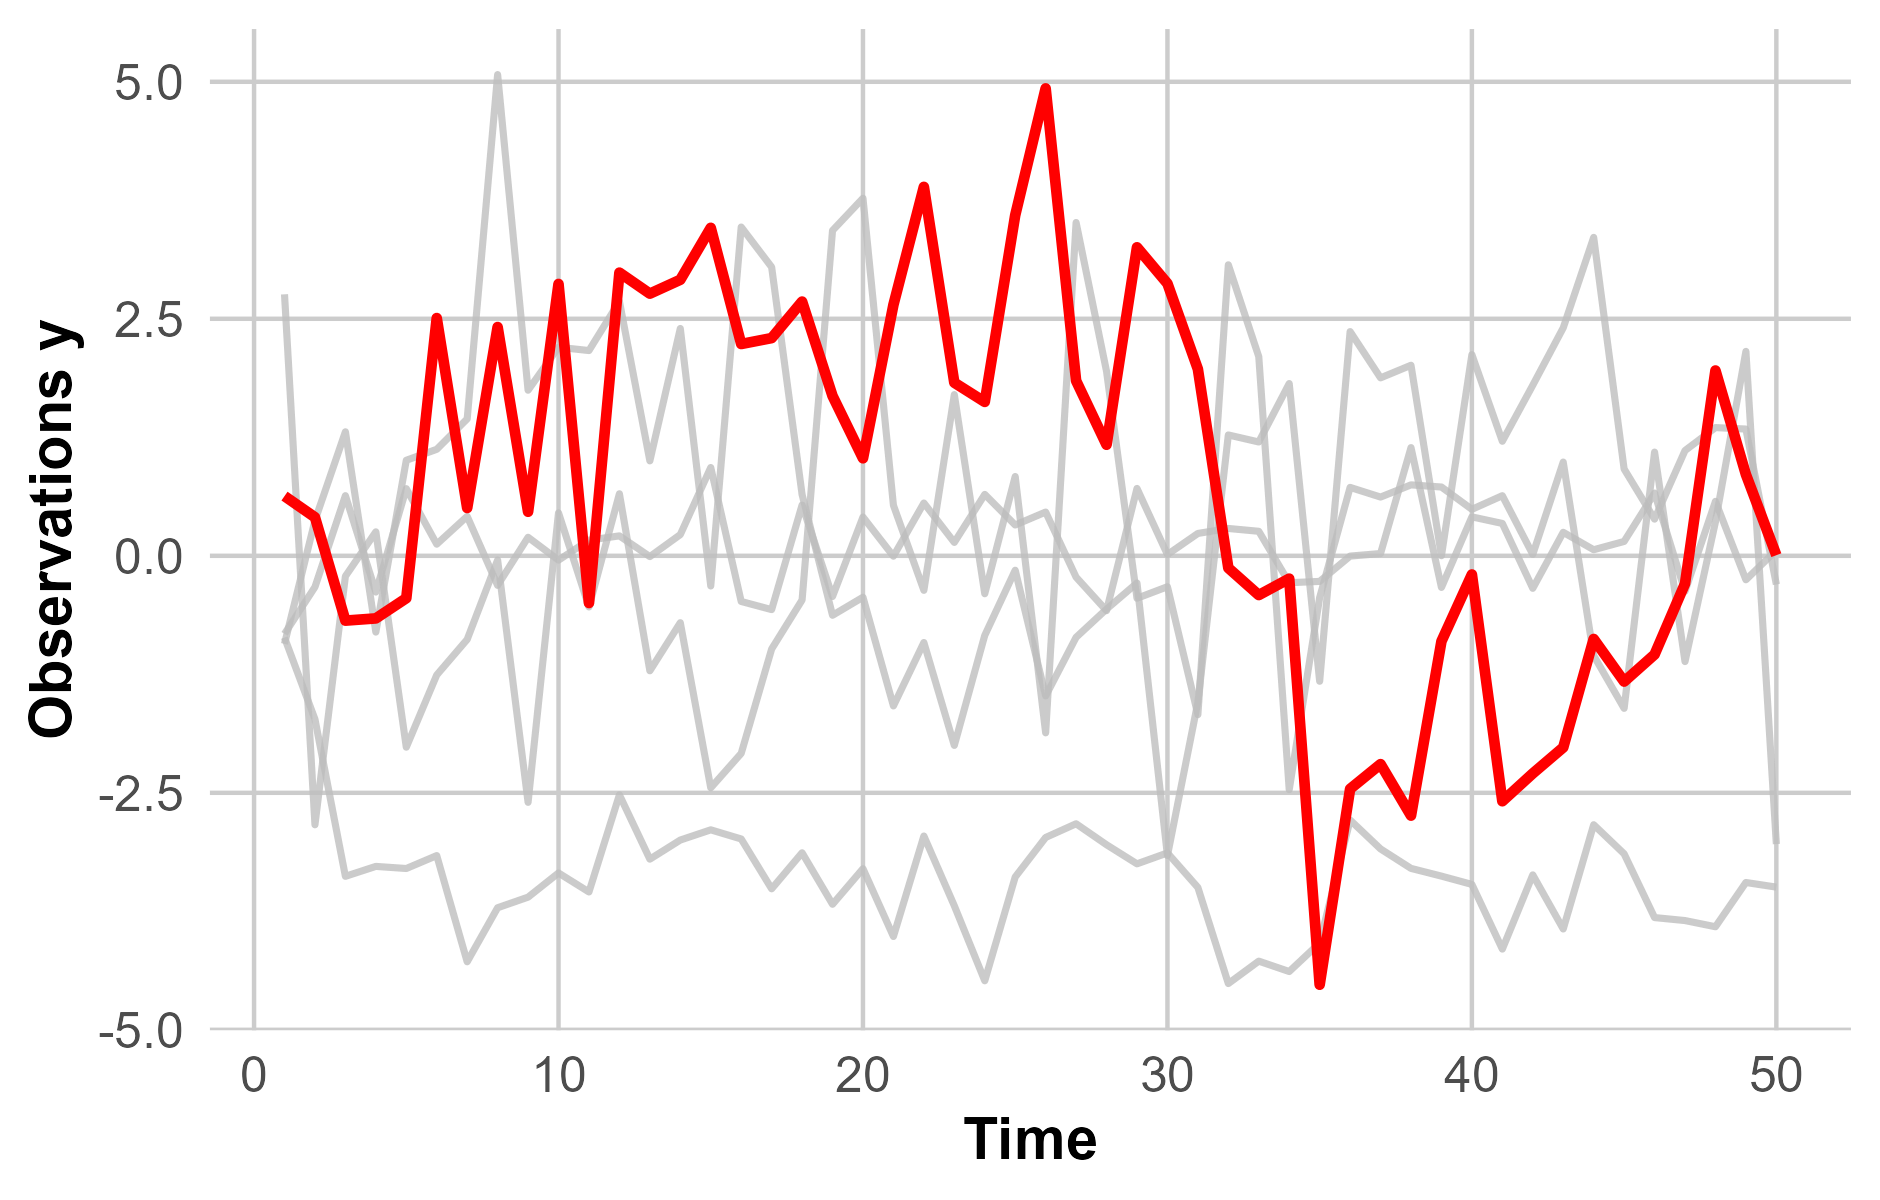
\includegraphics{prior_predictive_check.png}
		\caption{A simulated trajectory of the SSM in Example~\ref{exa:SSM_unknown_theta} alongside four simulated trajectories using the priors.}
		\label{fig:Prior_predictive_check}
		% Convert to pdf see https://www.overleaf.com/learn/latex/Inserting_Images Generating high-res and low-res images
	\end{figure}
	
	We use the proposal distribution
	\[
	q_{\text{pilot}}(\theta' \vert \theta) \sim N(\theta, 0.1 \cdot I),
	\]
	for a pilot run with $N_{\text{pilot}}=100$ particles and $M_{\text{pilot}}=2000$ \gls*{MCMC} iterations, discarding the first $1000$ samples as burn-in, and initializing $\theta$ from the priors. From this pilot run, we estimate both the posterior covariance matrix, $\hat{\mathcal{P}}$, and the posterior mean, $\hat{\theta}$. Next, using the estimated posterior mean, we calculate an estimate of the variance of the log-likelihood, denoted by $\widehat{\text{Var}}(\ell)$, by performing 10 repetitions with $N_{\text{pilot}}=100$ particles each time. Finally, we set
	\[
	N = \max\Bigl( N_{\text{pilot}} \cdot \widehat{\text{Var}}(\ell), \, 100 \Bigr),
	\]
	so that the log-likelihood has approximately unit variance at the estimated posterior while ensuring that $N$ is at least 100.
	
	We then run four independent \gls*{MCMC} chains with the proposal distribution
	\[
	q(\theta' \vert \theta) \sim N(\theta, \hat{\mathcal{P}}),
	\]
	for $M=15000$ \gls*{MCMC} iterations, discarding the first $2000$ samples as burn-in, using the value of $N$ from above and initializing $\theta$ as $\hat{\theta}$. The R code implementing this can be found at \url{https://github.com/BjarkeHautop/master-thesis/tree/main/R}; see also Appendix~\ref{chap:NumericalTricks} for further implementation details.
	
	An example chain is shown in Appendix~\ref{chap:supplementary_figures} in Figure~\ref{fig:chain}, where we see no clear signs that the chain has not converged and is not mixing well. To ensure that the posterior distribution produces data consistent with the observed data, we perform a posterior predictive check, shown in Figure~\ref{fig:Posterior_predictive_check}. The results appear reasonable, with the posterior values aligning well with the observed data.
	
	\begin{figure}
		\centering
		\textbf{Posterior predictive check}
		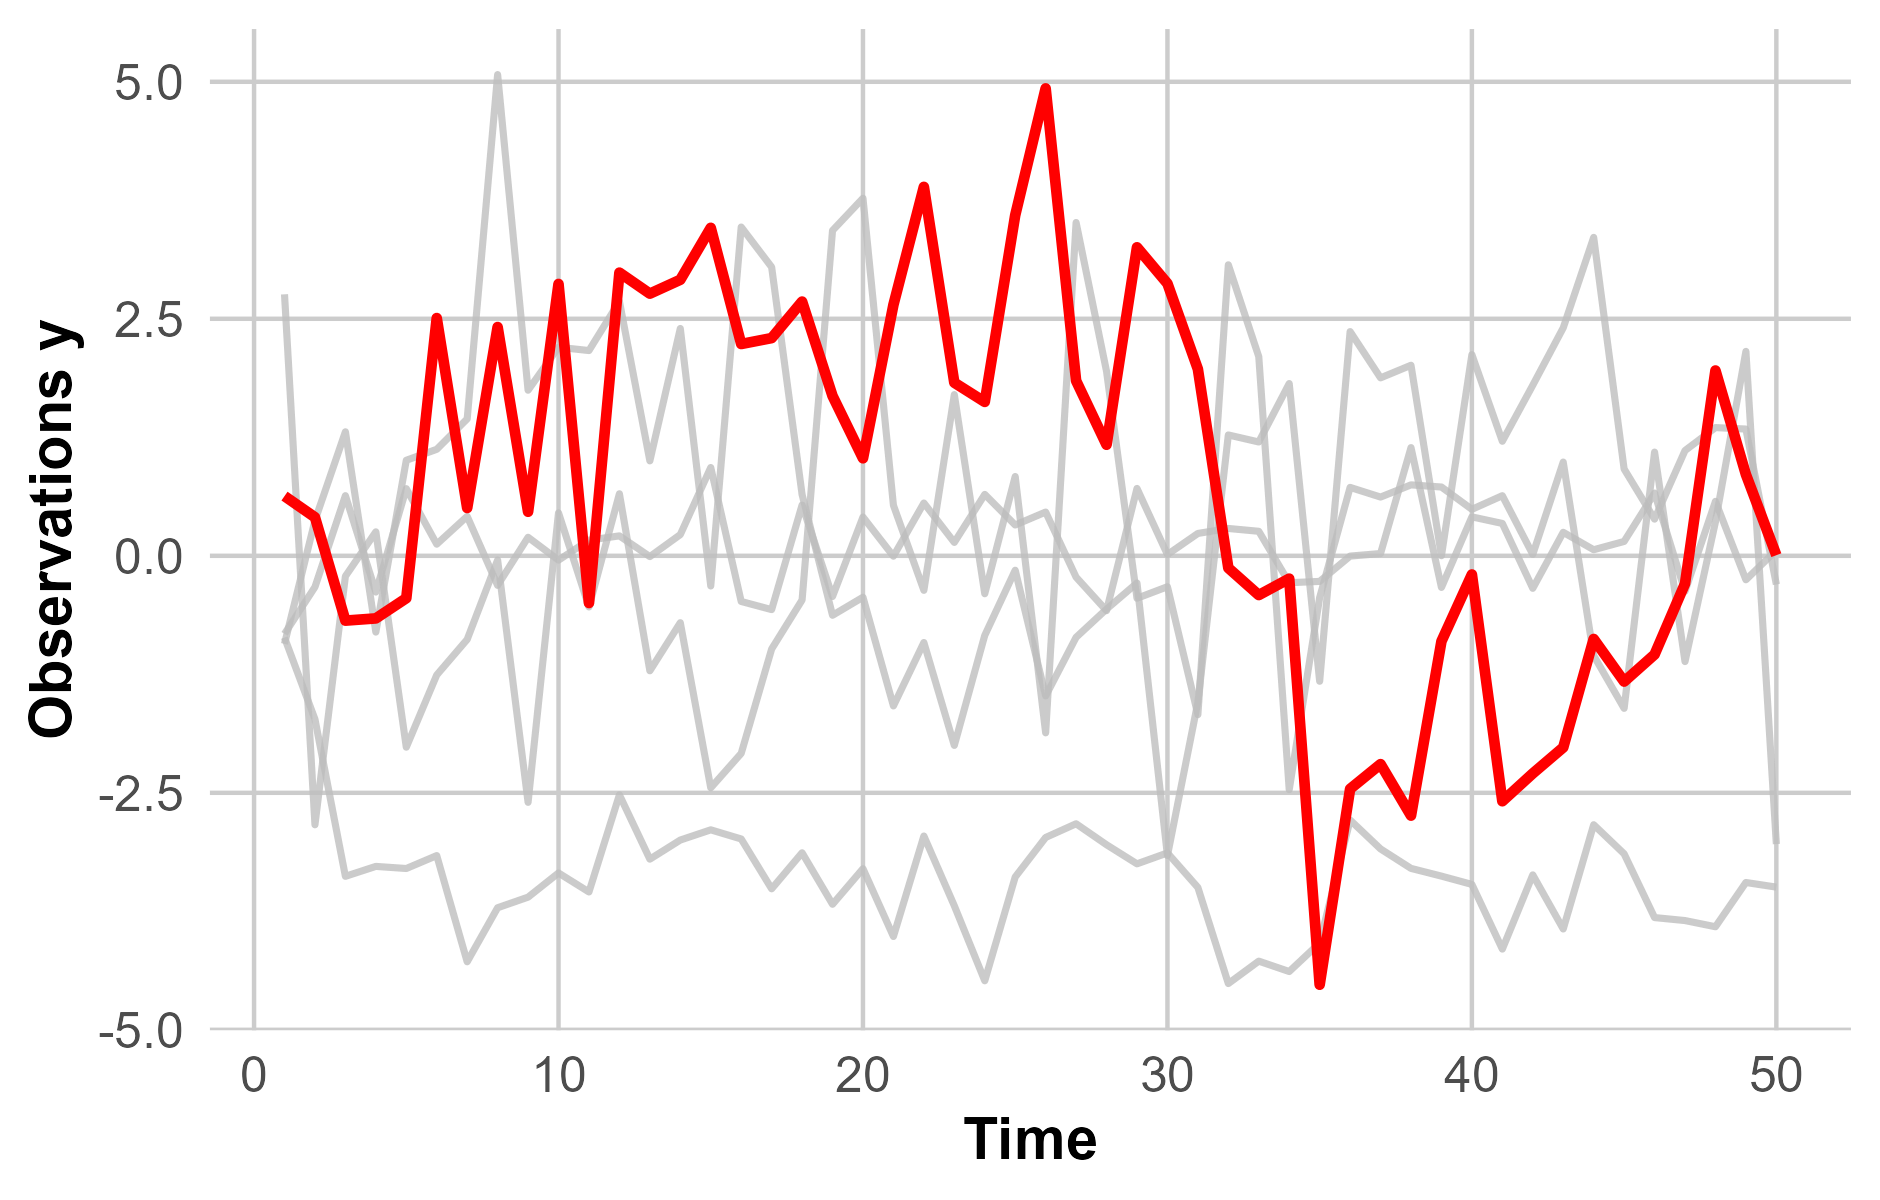
\includegraphics[width=\textwidth]{prior_predictive_check.png}
		\caption{A simulated trajectory of the SSM in Example~\ref{exa:SSM_unknown_theta} alongside four sample paths generated from the posterior predictive distribution.}
		\label{fig:Posterior_predictive_check}
		% Convert to pdf see https://www.overleaf.com/learn/latex/Inserting_Images Generating high-res and low-res images
	\end{figure} 
	
	To ensure that the chains agree and have converged to the same posterior we in Figure~\gls*{ESS} show the density plot of the four chains for $\phi$ (the figures for $\sigma_x$ and $\sigma_y$ can be found in \ref{chap:supplementary_figures}). We see that the four chains look very similar. We furthermore verify that we can trust the inference by computing the split-$\widehat{R}$ statistic and \gls*{ESS} (see Appendix~\ref{chp:appendixMCMC} for definition of these), which is summarized in Table~\ref{tab:diagnostics}. We see, that the ESS is much larger than the recommendation of at least 400 and the split-\(\widehat{R}\) are all below the recommended $1.01$. Thus, we can use the MCMC samples for reliable inference.
	
	\begin{figure}
		\centering
		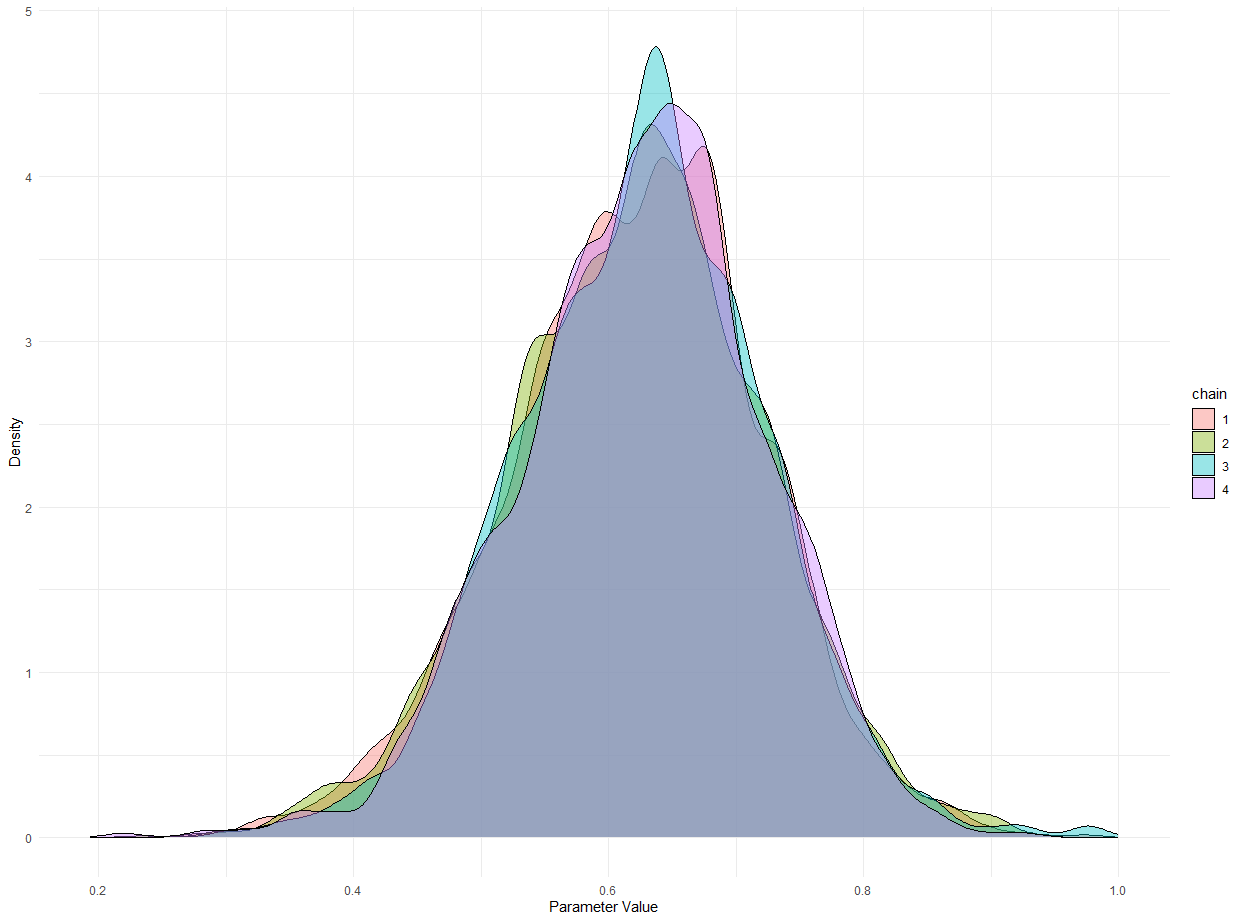
\includegraphics[width=\textwidth]{phi_density_plot.png}
		\caption{Density plot of the four chains for $\phi$ in Example~\ref{exa:SSM_unknown_theta}.
		\textbf{UPDATE FIGURE TO HIGH QUALITY}}
		\label{fig:phi_dens}
	\end{figure}
	
	\begin{table}
		\centering
		\caption{ESS and split-\(\widehat{R}\) for \(\phi\), \(\sigma_x\), and \(\sigma_y\)}
		\label{tab:diagnostics}
		\begin{tabular}{lcc}
			\toprule
			Parameter & ESS & split-\(\widehat{R}\) \\
			\midrule
			\(\phi\)       & 2609  & 1.002 \\
			\(\sigma_x\)   & 1806  & 1.002 \\
			\(\sigma_y\)   & 1304  & 1.003 \\
			\bottomrule
		\end{tabular}
	\end{table}
	
	The posterior mean and $95\%$ credible intervals are given in Table~\ref{tab:mean_credible_interval}. The RMSE of the latent state was $0.79$, only slightly worse than the result of the filtering and smoothing algorithms from Table~\ref{tab:performance_ext}, where the parameters were known. \textbf{ONLY BASED ON 1 SAMPLE}
	\begin{table}
		\centering
		\caption{Mean and Credible Interval for Parameters}
		\label{tab:mean_credible_interval}
		\begin{tabular}{lcc}
			\toprule
			Parameter & Mean & 95\% Credible Interval \\
			\midrule
			\(\phi\)       & 0.62  & [0.42, 0.81] \\
			\(\sigma_x\)   & 1.01  & [0.64, 1.49] \\
			\(\sigma_y\)   & 0.89  & [0.45, 1.29] \\
			\bottomrule
		\end{tabular}
	\end{table}
\end{example}



	
	% Chapter 5: Simulation Studies
	%\chapter{Simulation Studies}
	%\input{chapters/simulation.tex}
	
	% Chapter 6: Application to Stochastic SIR Models
	%\chapter{Application to Stochastic SIR Models}
	%\input{chapters/application.tex}
	
	% Chapter 7: Conclusion and Future Work
	%\chapter{Conclusion and Future Work}
	%\input{chapters/conclusion.tex}
	
	
	% Bibliography
	\bibliographystyle{abbrvnat}
	\bibliography{references}
	
	\appendix
	
	% Modify appendix
	\chapter{MCMC}
\label{chp:appendixMCMC}

Markov Chain Monte Carlo (MCMC) methods are used to generate samples from complex probability distributions when direct sampling is infeasible. Let $\pi(x)$ be a density that we want to sample from. An MCMC algorithm constructs a Markov chain $\{X_t\}_{t\geq 1}$ with transition kernel $P(x, A)$ which has $\pi(x)$ as stationary distribution. 

One widely used MCMC method is the Metropolis-Hastings algorithm. It generates a sequence of samples from $\pi(x)$ by proposing a candidate $x'$ from a proposal distribution $q(x'|x_t)$ based on the current state $x_t$. The candidate is accepted with probability:
\[
	\alpha = \min\left(1, \frac{\pi(x') q(x_t | x')}{\pi(x_t) q(x' | x_t)}\right)
\]
If the candidate is accepted, the next state is set to $x_{t+1} = x'$; otherwise, $x_{t+1} = x_t$. 

A key property ensuring that the chain has the desired stationary distribution is that the algorithm satisfies the detailed balance condition with respect to $\pi(x)$, that is
\[
	\pi(x_t)q(x'\vert x_t)\alpha(x_t, x')=\pi(x')q(x_t\vert x')\alpha(x', x_t),
\]
for all states $x_t$ and $x'$. Provided that the Markov Chain satisfies some required regularity conditions on the proposal distribution it has the correct stationary distribution. A sufficient condition is that 
\[\pi(x)>0 \implies q(x \vert x')>0 \quad \text{for any } x, x',\]
ensuring irreducibility, and that the chain is aperiodic (\cite{robert_monte_2004}).

%Let $f(x)$ be a function of interest and assume we generate a Markov chain $\{X_t\}$ with stationary distribution $\pi(x)$. The sample average

%\[
%	\widehat{\mu}_M = \frac{1}{M} \sum_{t=1}^{M} f(X_t)
%\]

%converges to the true expectation $\mathbb{E}_\pi[f(X)]$ under mild conditions.
In practice, when using \gls*{MCMC} methods for inference the first part of the chain is discarded to allow the chain to converge to the stationary distribution. This is referred to as \emph{burn-in}.

\section*{MCMC diagnostics}
Since convergence of \gls*{MCMC} is only guaranteed asymptotically, we must rely on diagnostic methods to assess convergence when working with a finite number of samples. Assume that we do MCMC to do inference about a parameter $\theta$, which, for ease of notation, we suppose is a scalar. For models involving multiple parameters, the diagnostic methods described below are applied to each parameter individually.
 
\subsection*{Potential Scale Reduction}
A method to evaluate the convergence of a \gls*{MCMC} chain is to run several independent chains and compare the behavior between them. This is the idea of the \emph{potential scale reduction statistic} $\widehat{R}$ first introduced in \cite{Rubin}. The potential scale reduction statistic compares the between-chain variance to the within-chain variance. If all chains are at equilibrium, these will be the same, and \(\widehat{R}\) will be one. If they haven't converged to a common distribution, the \(\widehat{R}\) statistic will be greater than one.

Suppose we have a set of $K$ Markov chains $\theta_k$ which each has $M$ samples $\theta_k^{(m)}$. The between-chain variance estimate is
\[
	B=\frac{M}{K-1}\sum_{k=1}^{K}(\overline{\theta}_k^{(\boldsymbol\cdot)}-\overline{\theta}_{\boldsymbol\cdot}^{(\boldsymbol\cdot)})^2,
\]
where $\overline{\theta}_k^{(\boldsymbol\cdot)}$ is the mean for chain $k$
\[
	\overline{\theta}_k^{(\boldsymbol\cdot)}=\frac{1}{M} \sum_{m=1}^M\theta_k^{(m)},
\]
and $\overline{\theta}_{\boldsymbol\cdot}^{(\boldsymbol\cdot)}$ is the overall mean of the chains
\[
	\overline{\theta}_{\boldsymbol\cdot}^{(\boldsymbol\cdot)}=\frac{1}{K}\sum_{k=1}^K \overline{\theta}_k^{(\boldsymbol\cdot)}.
\]
The within-chain variance is averaged over the chains,
\[
	W=\frac{1}{K}\sum_{k=1}^K s_k^2,
\]
where 
\[
	s_k^2=\frac{1}{M-1}\sum_{m=1}^M (\theta_k^{(m)}-\overline{\theta}_k^{(\boldsymbol\cdot)})^2.
\]
The variance estimator is given by a mixture of the within-chain and cross-chain sample variances,
\begin{equation}
	\widehat{\text{var}}^+(\theta)=\frac{M-1}{M}W+\frac{1}{M}B,
	\label{eq:var_est_rhat}
\end{equation}
This weighted combination accounts for the uncertainty in both the within-chain and between-chain variances. Finally, we can define the potential scale reduction statistic as
\[
	\widehat{R}=\sqrt{\frac{\widehat{\text{var}}^+(\theta)}{W}}.
\]
\cite{gelman2013bayesian} introduced split-$\widehat{R}$ as a more sensitive diagnostic for convergence in \gls*{MCMC} sampling. The method involves splitting each of the $K$ chains into two halves: the first $M/2$ samples and the last $M/2$ samples, giving $2K$ chains. The standard $\widehat{R}$ statistic is then computed across these $2K$ chains. By comparing the two halves of each chain, split-$\widehat{R}$ can detect issues such as slow mixing or nonstationarity within individual chains that might be overlooked when only comparing different chains.

A typical guideline is that $\widehat{R}$ values above $1.01$ indicates that further sampling is needed (\cite{Stan} and \cite{ImprovedhatR}).

\subsection*{Effective Sample Size} % NOT RELATED AT ALL TO OTHER EFFECTIVE SAMPLE SIZE FROM RESAMPLING
\textbf{Not the same or related to ESS for resampling condition in particle filter.}\newline
An $\widehat{R}$ close to $1$ does not guarantee that an MCMC sample is reliable (\cite{VatsKnudson}). A sufficiently large \gls*{ESS} is also required to obtain stable inferences for the quantities of interest. The MCMC samples will typically be positively autocorrelated within a chain. The \gls*{ESS} is the number of independent samples with the same estimation power as the $M$ autocorrelated samples. We follow the definitions given in \cite{Stan} and \cite{ImprovedhatR}.
% Estimation error 1/sqrt{N_eff} not 1/sqrt{N}.
\todo{SETUP}
We again let $K$ be the number of chains each consistent of $M$ samples and assume all the chains have reached the stationary distribution $p(\theta)$ with mean $\mu$ and variance $\sigma^2$. The autocorrelation $\rho_t$ at lag $t\geq 0$ is defined as
\begin{align*}
	\rho_t&=\frac{1}{\sigma^2}\int (\theta^{(n)}-\mu)(\theta^{(n+t)}-\mu)p(\theta)\, d\theta \\
	&=\frac{1}{\sigma^2}\int \theta^{(n)}\theta^{(n+t)}p(\theta)\, d\theta,
\end{align*}
where we used that $\theta^{(n)}$ and $\theta^{(n+t)}$ have the same stationary distribution. We then define the effective sample size $M_{\text{eff}}$ of $M$ samples by
\[
	M_{\text{eff}}=\frac{M}{1+2\sum_{t=1}^{\infty}\rho_t}.
\]
For independent draws (i.e., \(\rho_t = 0\) for \(t \ge 1\)), we recover \(M_{\text{eff}}=M\). 
When draws are positively correlated, however, \(M_{\text{eff}}\) is smaller, reflecting the reduced information content of the chain, while if they were negatively correlated, the effective sample size will exceed the number of iterations. The \gls*{ESS} is a particular important measure, since the standard error of the estimate of a parameter decreases by $1/\sqrt{M_\text{eff}}$ and not $1/\sqrt{M}$.
 
In practice, the integral of the joint distribution $p(\theta)$ is intractable and thus we need to estimate the effective sample size. We can estimate the autocorrelation $\rho_t$ by
\[
	\hat{\rho}_t=1-\frac{W-\frac{1}{K}\sum_{k=1}^K\hat{\rho}_{t,k}}{\widehat{\text{var}}^+(\theta)},
\]
where $\hat{\rho}_{t,k}$ is an estimate of the autocorrelation at lag $t$ for the $k$th Markov chain, and $\widehat{\text{var}}^+(\theta)$ is defined in Equation~(\ref{eq:var_est_rhat}). Because of the increased noise of $\hat{\rho}1_{t}$ as $t$ increases, in practice a truncated sum of $\hat{\rho}_t$ is used. We apply Geyer’s initial monotone sequence criterion, as defined in \cite{Geyer1992}, to ensure stability. The effective sample size is estimated by 
\[
	\widehat{M}_{\text{eff}}=\frac{KM}{\hat{\tau}},
\]
where
\[
	\hat{\tau}=1+2\sum_{t=1}^{2k+1}\hat{\rho}_t=1+2\sum_{t=0}^m \hat{P}_{t}-\hat{\rho}_0=-1+2\sum_{t=0}^m \hat{P}_{t},
\]
where $\hat{P}_{t}=\hat{\rho}_{2t}+\hat{\rho}_{2t+1}$. Summing over pairs starting from lag 0 ensures that the sequence 
$\hat{P}_t$ values is non-negative and non-increasing (\cite{Geyer1992}). So, if we observe negative estimates of the autocorrelations it is due to finite-sample noise. Thus, we define an initial positive sequence by choosing the largest $m$ such that $\hat{P}_t>0$ for all $t \in \{1,\dots,m\}$. We also enforce monotonicity by modifying the sequence $\hat{P}_t$ so that it does not exceed the smallest preceding value, ensuring a non-increasing sequence.

\chapter{Bayesian model validation}
\label{chap:Bayesian_model_val}
This Chapter contains some common tools used for validating a Bayesian model.
\section*{Prior predictive check}
Before fitting a Bayesian model it is useful to assess whether the prior distributions are reasonable in the context of the model. This can be done using a prior predictive check, where data is simulated using parameters drawn from the prior. If the generated data is implausible, it suggests that the priors may be too weakly or strongly informative.

\section*{Posterior predictive check}
After fitting a Bayesian model a posterior predictive check is used to evaluate how well the fitted model explains the observed data. Here, data is simulated using parameter values sampled from the posterior distribution. If the replicated data fails to resemble the observed data, it suggests that the model may not capture key aspects of the underlying data-generating process.

\section*{Prior Sensitivity Analysis}
Prior sensitivity analysis is assessing how sensitive the model’s inferences are to the choice of prior distributions. It involves re-running the model with different reasonable priors and comparing the resulting posterior distributions. This analysis helps determine how large of an effect the prior has on the posterior.

Since it is expensive to fit the same model many times with different priors, in practice it is often done using importance sampling, see for example \cite{vehtari2024paretosmoothedimportancesampling}.

\chapter{Numerical stability tricks}
\label{chap:NumericalTricks}
This is a collection of some of the numerical tricks used in the implementation of the algorithms to avoid underflow and improve efficiency. 

\section*{Log-Sum-Exp Trick}
When aggregating the contributions of multiple particles to the log-likelihood, we need to compute a sum of the form
\[
	L_t = \frac{1}{N}\sum_{i=1}^N \exp(\ell_i),
\]
where \(N\) is the number of particles and $\ell_i$ is the $\log$-weights. Direct exponentiation of \(\ell_i\) can lead to numerical underflow if \(\ell_i\) is very small. To mitigate this, we use the log-sum-exp trick (\cite{Stan}).
Define
\[
	M = \max_{1 \le i \le N} \ell_i.
\]
Then,
\[
	\log\left(\sum_{i=1}^N \exp(\ell_i)\right) = M + \log\left(\sum_{i=1}^N \exp(\ell_i - M)\right).
\]
Thus, the incremental log-likelihood is computed as
\[
\log L_t = -\log N + M + \log\left(\sum_{i=1}^N \exp(\ell_i - M)\right).
\]
This approach rescales the log-likelihoods so that the exponential terms do not vanish numerically.

\section*{Transformation of Parameters}
When parameters are defined on constrained domains, it is often beneficial to transform them into an unconstrained space to facilitate efficient MCMC proposals. Using a standard proposal distribution, such as the normal distribution, directly in the constrained space can lead to proposed values that lie outside the domain, resulting in a likelihood of zero. Suppose we have a vector of parameters 
\[
	\theta = (\theta_1, \theta_2, \dots, \theta_n)
\]
where some components are defined on a constrained domain. For those components that are already unconstrained, we simply use the identity mapping, i.e., 
\[
	g_i(\theta_i)=\theta_i.
\]
For the constrained parameters, we introduce an invertible and differentiable transformation \(g_i\) that maps the constrained \(\theta_i\) into an unconstrained space:
\[
	\phi_i = g_i(\theta_i), \quad i = 1,2,\dots,n.
\]
A common example is proposing values for a standard deviation, which must be positive, and we can then instead propose values in $\log$-space.

If \(p(\theta)\) denotes the joint density of \(\theta\) and \(\theta_i = g_i^{-1}(\phi_i)\) is the inverse transformation, the joint density in the \(\phi\)-space is given by the change-of-variables formula:
\[
	p_{\phi}(\phi) = p\bigl(g_1^{-1}(\phi_1), \dots, g_n^{-1}(\phi_n)\bigr) \prod_{i=1}^n \left|\frac{d}{d\phi_i} g_i^{-1}(\phi_i)\right|.
\]
Taking logarithms yields the transformed log density:
\[
	\log p_{\boldsymbol{\phi}}(\boldsymbol{\phi}) = \log p\bigl(g_1^{-1}(\phi_1), \dots, g_n^{-1}(\phi_n)\bigr) + \sum_{i=1}^n \log\left|\frac{d}{d\phi_i} g_i^{-1}(\phi_i)\right|.
\]


\chapter{Supplementary Figures}
\begin{figure}
	\centering
	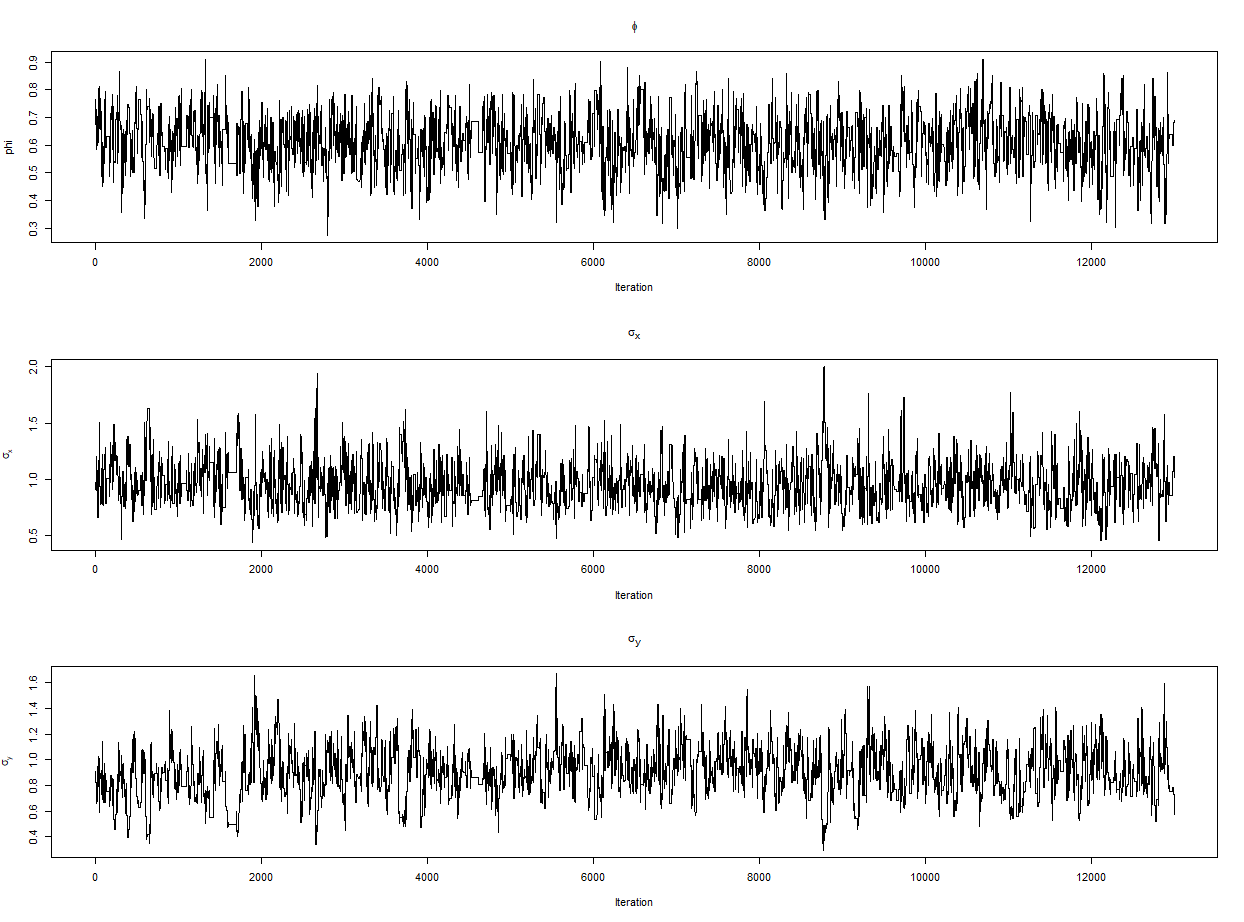
\includegraphics[width=1\textwidth]{chain_plot.png}
	\caption{A trace plot of an MCMC chain for the parameter vector $\theta=(\phi, \sigma_x, \sigma_y)$ in Example~\ref{exa:SSM_unknown_theta}\textbf{UPDATE FIGURE TO HIGH QUALITY}}
	\label{fig:chain}
	% Convert to pdf see https://www.overleaf.com/learn/latex/Inserting_Images Generating high-res and low-res images
\end{figure} 

\label{chap:supplementary_figures}
\begin{figure}
	\centering
	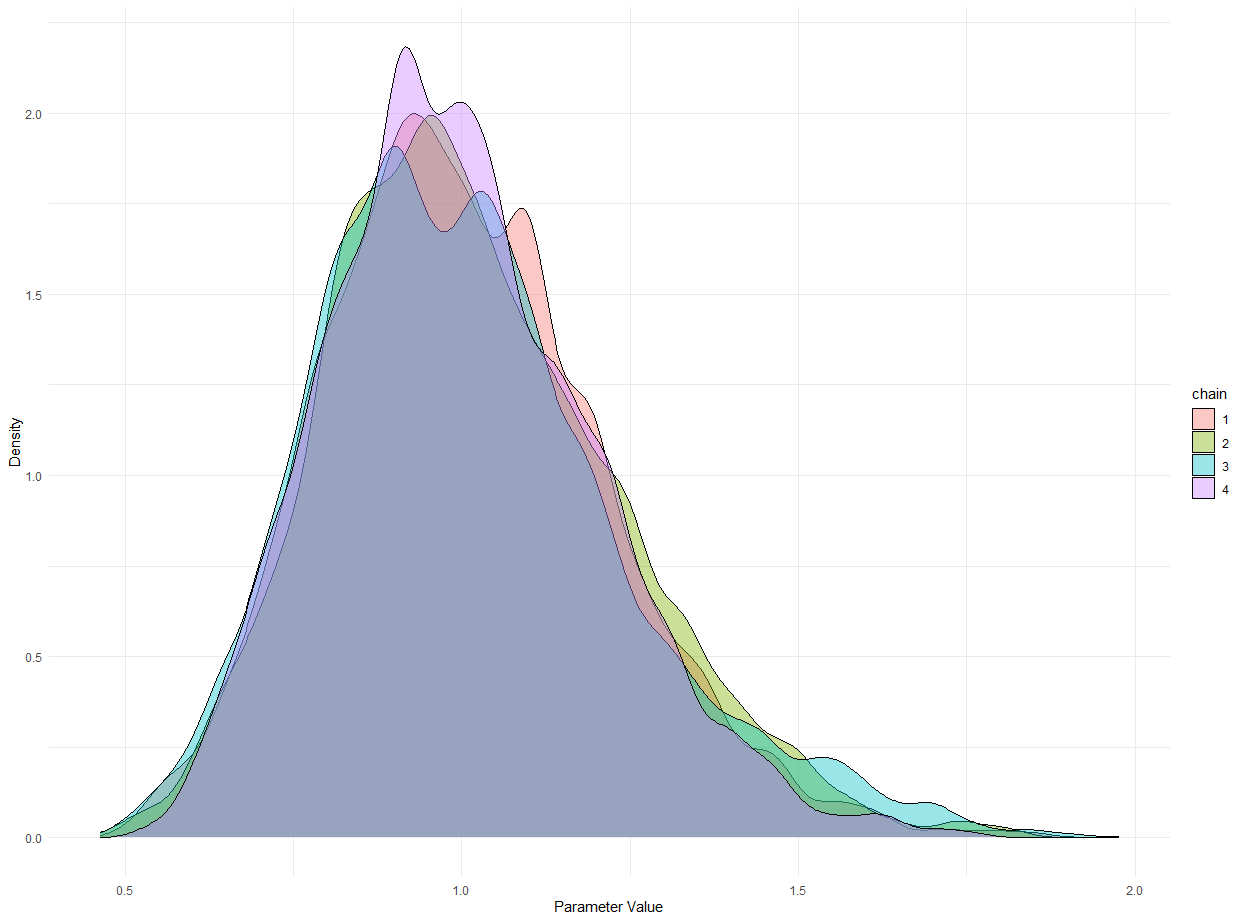
\includegraphics[width=\textwidth]{sigma_x_density_plot.png}
	\caption{Density plot of the four chains for $\sigma_x$ in Example~\ref{exa:SSM_unknown_theta}\textbf{UPDATE FIGURE TO HIGH QUALITY}}
	\label{fig:sigma_x_dens}
\end{figure}

\begin{figure}
	\centering
	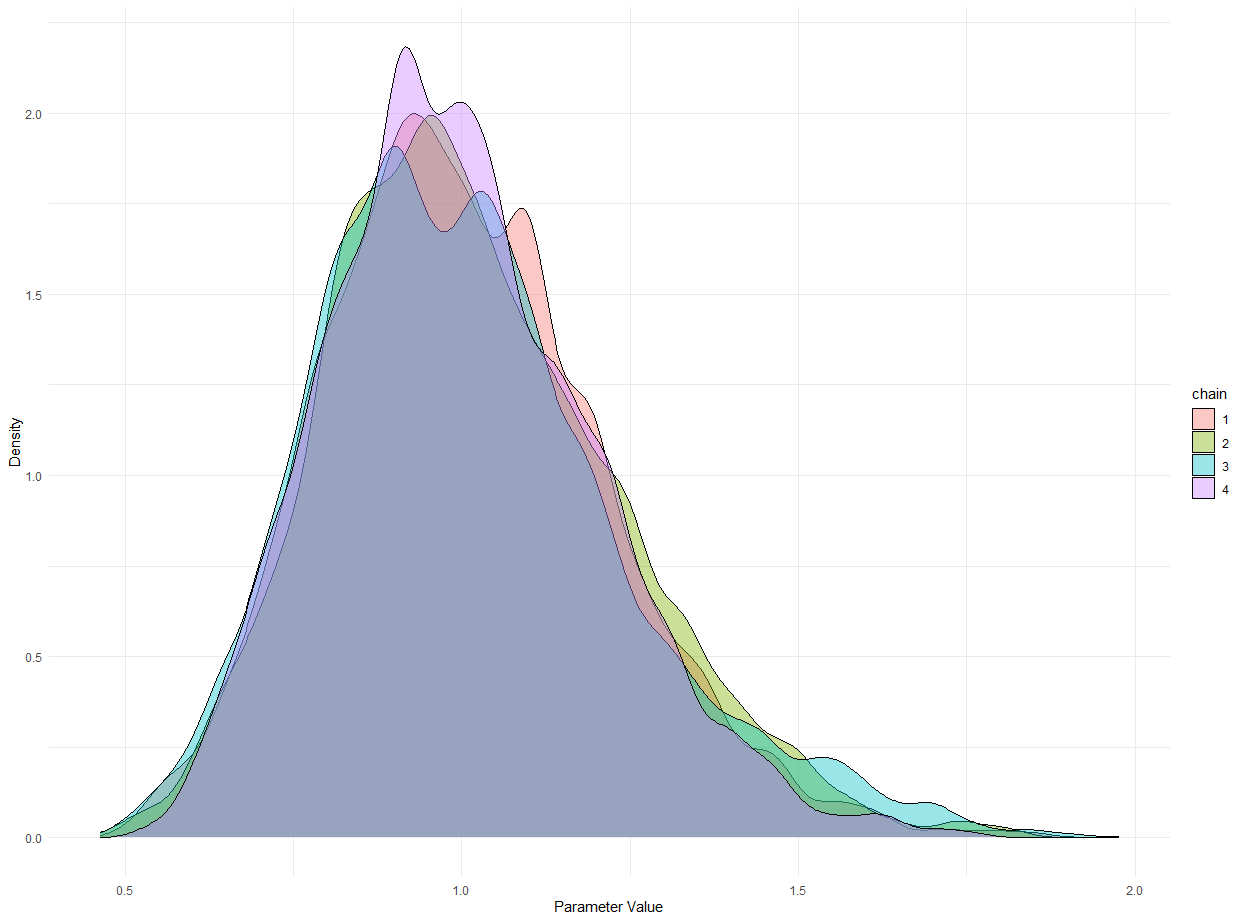
\includegraphics[width=\textwidth]{sigma_x_density_plot.png}
	\caption{Density plot of the four chains for $\sigma_y$ in Example~\ref{exa:SSM_unknown_theta}\textbf{UPDATE FIGURE TO HIGH QUALITY}}
	\label{fig:sigma_y_dens}
\end{figure}
	
	
	
\end{document}
